\begin{surferPage}{Eine $A_5^{--}$ Singularität}
 Eine Fläche heißt nicht-singulär oder glatt, wenn sie, anschaulich gesagt,
    keine spitzen Stellen (Singularitäten genannt) hat, z.B.\ eine Kugel, 
    ein Torus (1.\ bzw.\ 2.\ Bild von links):
    \begin{center}
      \vspace{-0.2cm}
      \begin{tabular}{@{}c@{}c@{}c@{}c@{}}
        \begin{tabular}{@{}c}
          \includegraphics[width=1.1cm]{../../common/images/kugel}
        \end{tabular}
        &
        \begin{tabular}{@{}c}
          \includegraphics[width=1.1cm]{../../common/images/torus}
        \end{tabular}
        &
        \begin{tabular}{c@{}}
          \includegraphics[width=1.1cm]{../../common/images/kegel}
        \end{tabular}
        &
        \begin{tabular}{c@{}}
          
\includegraphics[width=1.1cm]{../../common/images/A2pm_ill}
        \end{tabular}
      \end{tabular}
    \end{center}
    \vspace{-0.2cm}
    Die sogenannten ADE-Singularitäten sind die einfachsten Singularitäten.  
    Beispiele sind Singularitäten vom Typ $A_k^{\pm\pm}$ mit Gleichung
    $x^{k+1}\pm y^2\pm z^2$. 
    Bild rechts: $A_2^{+-}$, daneben: $A_1^{+-}$ (auch Doppelkegel genannt).

    Die ADE-Singularitäten haben ganz erstaunliche Beziehungen 
    zu unzähligen anderen Gebieten der Mathematik, Physik sowie belebter
    und unbelebter Natur, die bis heute nicht völlig verstanden sind.

    Jede $A_k$-Singularität lässt sich in $[\frac{k+1}{2}]$
    $A_1$-Singularitäten deformieren; für $A_5^{--}$ (großes Bild) ergeben
    sich drei $A_1$-en: 
%    \dontshow{
    % 
    \begin{center}
      \vspace{-0.1cm}
      \begin{tabular}{@{}c@{\quad}c@{\quad}c@{}}
        \begin{tabular}{@{}c@{}}
          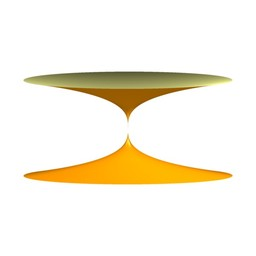
\includegraphics[width=1.2cm]{../../common/images/A5mm_0}
        \end{tabular}
        &
        \begin{tabular}{@{}c@{}}
          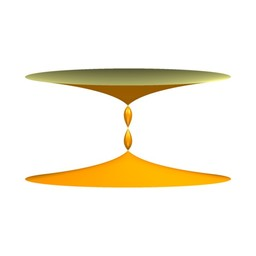
\includegraphics[width=1.2cm]{../../common/images/A5mm_1}
        \end{tabular}
        &
        \begin{tabular}{@{}c@{}}
          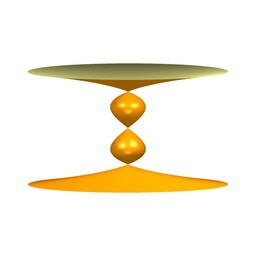
\includegraphics[width=1.2cm]{../../common/images/A5mm_2}
        \end{tabular}
      \end{tabular}
    \end{center}
%    }
 
\end{surferPage}
